\documentclass[11pt]{standalone}

\usepackage{helvet}

\usepackage{ifthen}
\usepackage{tikz} 
\usetikzlibrary{shapes.misc}
\usetikzlibrary{arrows,arrows.meta}
\usetikzlibrary{calc,intersections, patterns, math}

\definecolor{pfeil}{RGB}{168,167,167}
\definecolor{petrol}{RGB}{0, 118, 136}
\definecolor{darkgoldenrod}{RGB}{184, 134, 11}
\colorlet{petrol-lighter}{petrol!40}
\colorlet{darkgoldenrod-lighter}{darkgoldenrod!40}

\begin{document}

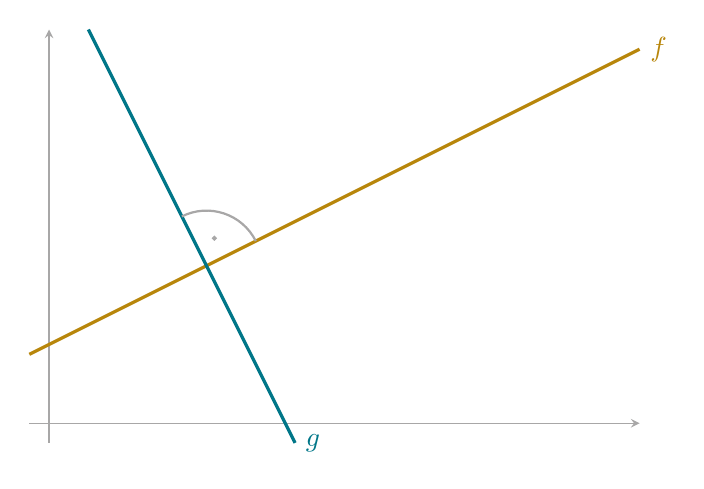
\begin{tikzpicture}[pfeil]

    % \draw[thick, fill=petrol!20, draw=petrol-lighter, rounded corners=2ex, opacity=0.5] (0,0) rectangle ++ (1.5,3.5);
    % \draw[thick, fill=darkgoldenrod!20, draw=darkgoldenrod-lighter, rounded corners=2ex, opacity=0.5] (5,0) rectangle ++ (1.5,3.5);

    \draw[-stealth] (-0.25,0) -- (7.5,0);
    \draw[-stealth] (0,-0.25) -- (0,5);
    \draw[very thick, darkgoldenrod] (-0.25,0.875) -- (7.5,4.75) node[right] {$f$};
    \draw[very thick, petrol] (0.5,5) -- (3.125,-0.25) node[right] {$g$};

    \draw[thick] (2,2)++(26.57:0.7) arc(26.57:116.57:0.7);
    \draw[fill] (2.1,2.35) circle (0.025);
    

\end{tikzpicture}

\end{document}
